%%%%%%%%%%%%%%%%%%%%%%%%%%%%%%%%%%%%%%%%%%%%%%%%%%%
%
%  New template code for TAMU Theses and Dissertations starting Fall 2016.  
%
%
%  Author: Sean Zachary Roberson
%  Version 3.17.09
%  Last Updated: 9/21/2017
%
%%%%%%%%%%%%%%%%%%%%%%%%%%%%%%%%%%%%%%%%%%%%%%%%%%%

%%%%%%%%%%%%%%%%%%%%%%%%%%%%%%%%%%%%%%%%%%%%%%%%%%%%%%%%%%%%%%%%%%%%%%%
%%%                           SECTION II
%%%%%%%%%%%%%%%%%%%%%%%%%%%%%%%%%%%%%%%%%%%%%%%%%%%%%%%%%%%%%%%%%%%%%%


\chapter{METHODS} 
\section{Basic Altimeter Test Bed Setup} \label{sec:Basic}
In addition to laying out performance standards for radar altimeters, the DO-155 standards~\cite{noauthor_minimum_1974} also specify a basic test setup for verifying an altimeter is functioning properly. Figure~\ref{fig:Basic Testbed} shows the diagram of this test setup. The standards also elaborated on the necessary characteristics of the most critical part of the testbed, the altitude simulator. 

The altitude simulator needed to ''consist of variable and fixed RF attenuators''~\cite{noauthor_minimum_1974}  to simulate the loop loss an altimeter experiences aboard an aircraft (see section 1.6.3). The altitude simulator also needed a length of ''coaxial cables or other suitable delays''~\cite{noauthor_minimum_1974}  to simulate the physical time delay experienced by an altimeter signal between the transmitter and receiver (see section 1.6.2). To complete the test setup, the altitude simulator directed the attenuated and delayed RF energy from the transmitter fed back into the receiver. 
\begin{figure}[ht]
\centering
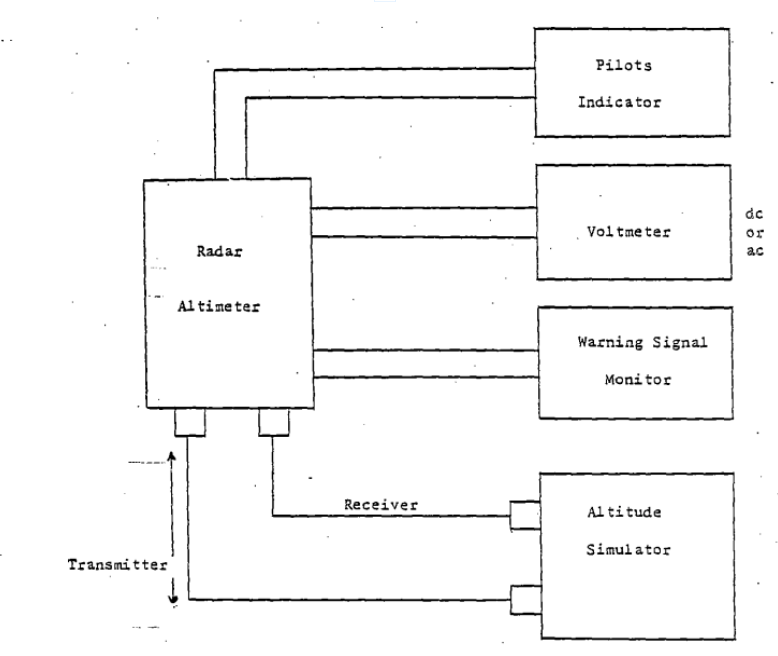
\includegraphics[scale=0.5]{DO-155_Test_Setup.PNG}
\caption[]{Basic Altimeter Test Setup from DO-155~\cite{noauthor_minimum_1974}}

\label{fig:Basic Testbed}

\end{figure}

Additionally, the standards specified that any test equipment must account for cross coupling between transmitting and receiving antennas. DO-155 emphasized that the altitude simulator should achieve the desired altitude within 1\% and the correct attenuation within 2.5dB~\cite{noauthor_minimum_1974}.

\section{Modified Altimeter Test Setup} \label{sec:Modified}
AVSI designed a modified version of the altimeter test setup specified by DO-155, shown in Figure~\ref{fig:Modified}. The modifications allow the controlled injection of interference into the line after the altimeter signal passes  through the altitude simulator. 

\begin{figure}[ht]
\centering
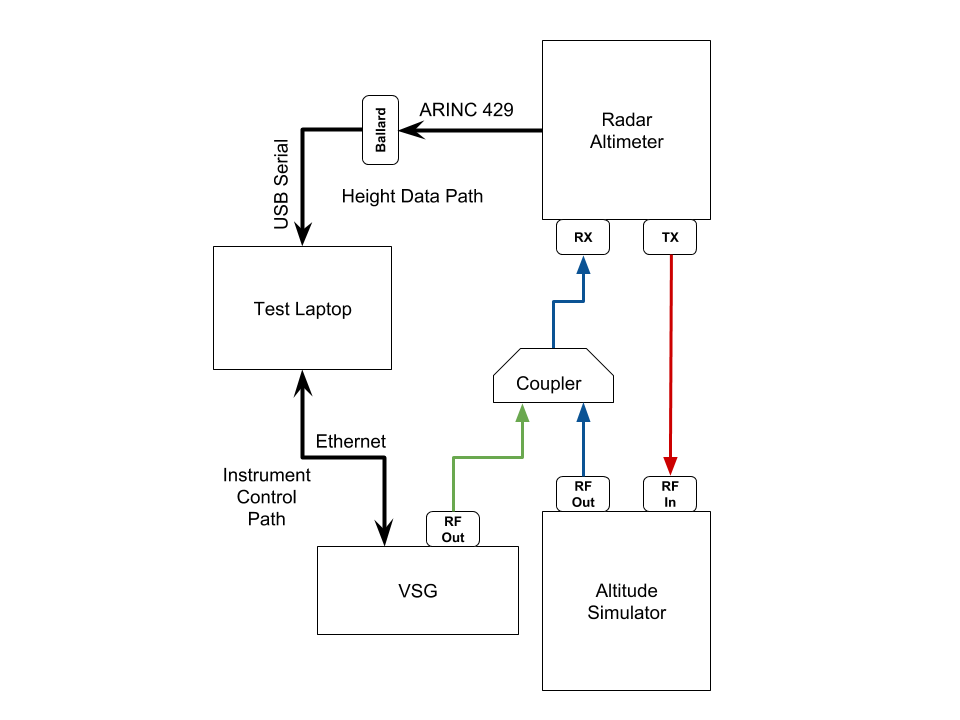
\includegraphics[scale=0.45]{Modified_Test_Setup.png}
\caption[]{Modified Altimeter Test Setup}

\label{fig:Modified}

\end{figure}
\subsection{Reading the Altimeter Output}\label{sub:reading_out}
The altimeter outputs labeled height data on a standardized ARINC 429 cable configuration. The modified setup uses a Ballard ARINC device to convert the data from ARINC 429 to USB serial format, providing each data point with a time stamp. On the test laptop, Ballard CoPilot software reads the serial data and provides a display which allows the real time monitoring of all altimeter output and labels. The labels are critical because some data points may be labeled NCD, or No Computed Data, when conditions are insufficient for a reliable height measurement. CoPilot software also allows for the easy export of test data to Microsoft Excel documents for post processing. 
\subsection{Implementing the Altitude Simulator}\label{sub:Implementing}
\subsubsection{Time Delay}\label{subsub:delay}
Different test altitudes required the use of different methods of delaying the RF energy output by the altimeters. For higher altitude tests, spools of fiber optic cables created a time delay. The RF output from the altimeter transmitter was fed by coax connection to the fiber optic transceiver, which could either pass the signal to a single fiber optic spool or a series of cascaded spools to achieve a desired height. This setup contained optical spools of 500, 1000, 2000, and 4500 feet, each of which could be used individually or in conjunction with any or all of the other spools to implement a delay.

 The optical transceiver and cascaded spools also contribute an attenuation to the loop loss which varies based on the number of spools cascaded. A single spool setup has an attenuation verified experimentally to be 29dB, with an additional 2dB loss added for each additional cascaded spool.

Later tests would modify this delay setup to test an altimeter in takeoff and landing scenarios. The much lower height in these scenarios meant that a spool of coax could be used tor the delay instead of fiber optic cables. Two coax spools provided a height of 40 ft and 95 ft for testing these scenarios, with a 6dB and 36dB attenuation contributed to the loop loss respectively.  

\subsubsection{Achieving Standard Loop Losses}\label{subsub:loss}
DO-155 specifies loop loss for various heights and antenna types. For these tests, the loop loss used for each height is listed in Table~\ref{tab:loop loss} To achieve the Loop Losses specified by DO-155 standards for each height, the attenuation inherent in the delay method used for each height must be taken into account. Once the attenuation from the delay line is subtracted from the loop loss, 10, 20 and 30dB Pasternack fixed attenuators are inserted into the setup to get within 10dB of the desired loop loss. These are located within the setup in part to protect the fiber optic transceiver from damage.  Finally, a step attenuator capable of 1 to 11 dB is used to achieve the desired loop loss with a 1 dB precision. 

\begin{table}[]
\centering
\begin{tabular}{|c|c|}
\hline
\textbf{Height} & \textbf{Loop Loss} \\ \hline
40ft            & 76 dB              \\ \hline
95ft            & 84 dB              \\ \hline
500ft           & 100 dB             \\ \hline
1500ft          & 109 dB             \\ \hline
3000ft          & 116 dB             \\ \hline
5000ft          & 120 dB             \\ \hline
8000ft          & 124 dB             \\ \hline
\end{tabular}
\caption{DO-155 Loop Losses}
\label{tab:loop loss}
\end{table}

\subsection{Generating Interference Signals}\label{sub:Generating}
A Rhode and Schwarz SMU200A Vector Signal Generator (VSG) is used to generate simulated WAIC signals of varying modulation types, bandwidths and power levels. The VSG has a SCPI interface which allows an external computer to control any functionality on the instrument through commands sent over either a serial or an Ethernet connection. 
\begin{figure}[ht]
\centering
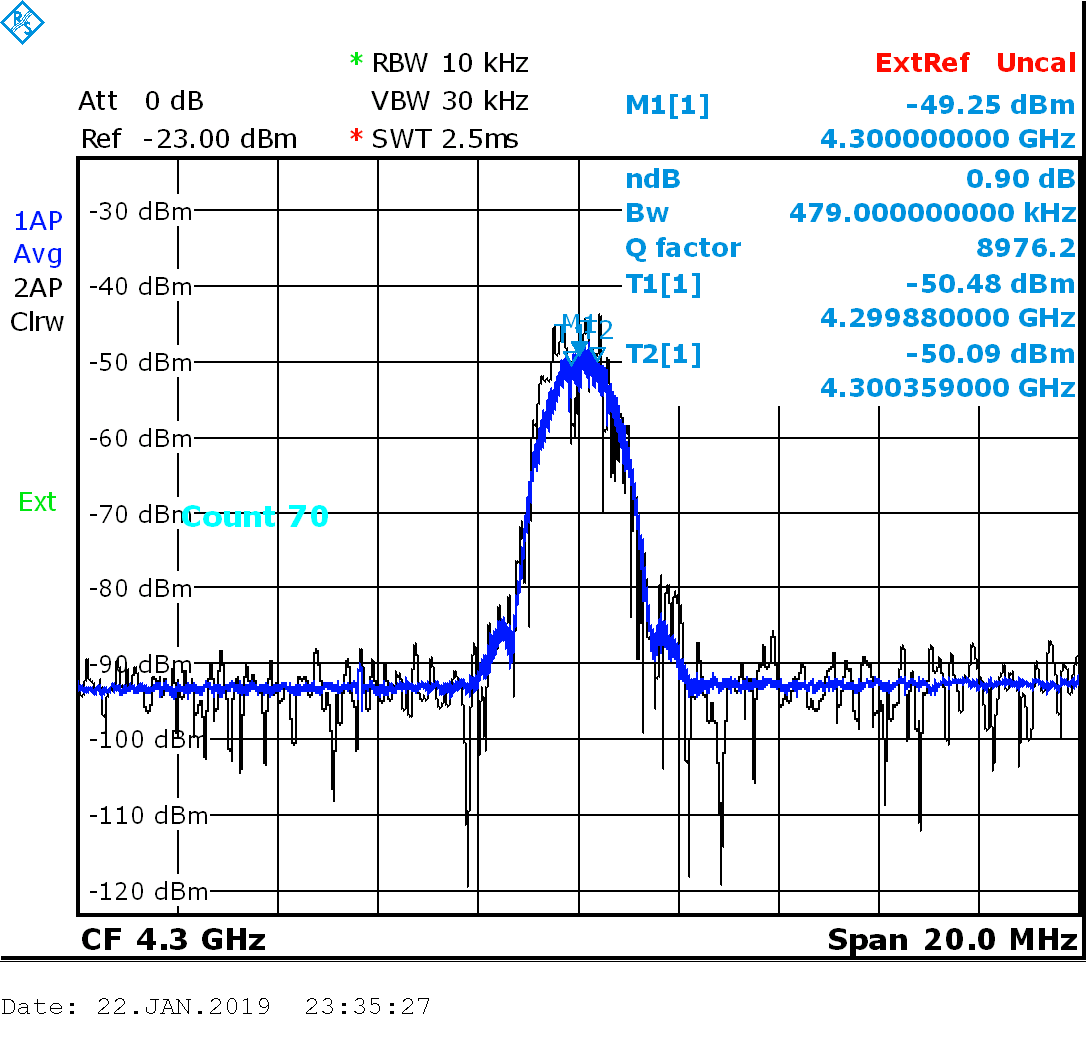
\includegraphics[scale=0.25]{MSK_wvfrm.png}
\caption[]{MSK Waveform at 4.3 GHz Pictured on a Spectrum Analyzer}

\label{fig:MSK}

\end{figure}
Modulation formats were chosen by the AFE76 Project Management Committee (PMC). The PMC chose to subject the altimeters to an MSK waveform modulated onto a wave form, as well as OFDM waveforms of varying bandwidths. The PMC also chose to use dual versions of both these waveforms. Both waveforms used ''junk'' data to modulate the carrier, which consisted of randomly generated ones and zeros with equal probability of either, which have been shown to closely replicate the performance of an optimal communication system [need citation]~\cite{}
\subsubsection{MSK Waveform}\label{subsub:MSK}
MSK or Minimum-Shift Keying is a type of modulation format which can be considered as a form of Phase-Shift Keying (PSK) or as a special case of Frequency Shift Keying (FSK)~\cite{proakis_communication_2002}. The frequency separation of an MSK signal, $\Delta f$ is: $$ \Delta f = \frac{1}{2T}$$
and thus it has a modulation index of 1/2. This is ''the minimum frequency separation for orthogonality of the two sinusoids''~\cite{proakis_communication_2002}. An MSK waveform is shown on the spectrum analyzer screen-cap in Figure~\ref{fig:MSK}.

MSK modulation is available natively through the VSG software. Through the \textit{custom waveform} interface, the Rhode and Schwarz VSG provides a number of common modulation options for the user to choose from. This simplifies the waveform generation for this case, as every in-built functionality on the VSG has a SCPI command corresponding to it. 


\subsubsection{OFDM Waveform}\label{subsub:OFDM}

Orthogonal Frequency-Division Multiplexing or OFDM attempts to achieve an efficient, wide-bandwidth communication system by ''dividing the channel bandwidth into equal-bandwidth sub-channels, where the bandwidth of each sub-channel is sufficiently narrow so that the frequency response... of sub-channels are nearly ideal''~\cite{proakis_communication_2002}. An OFDM waveform is shown on the spectrum analyzer screen-cap in Figure~\ref{fig:OFDM}.
\begin{figure}[ht]
\centering
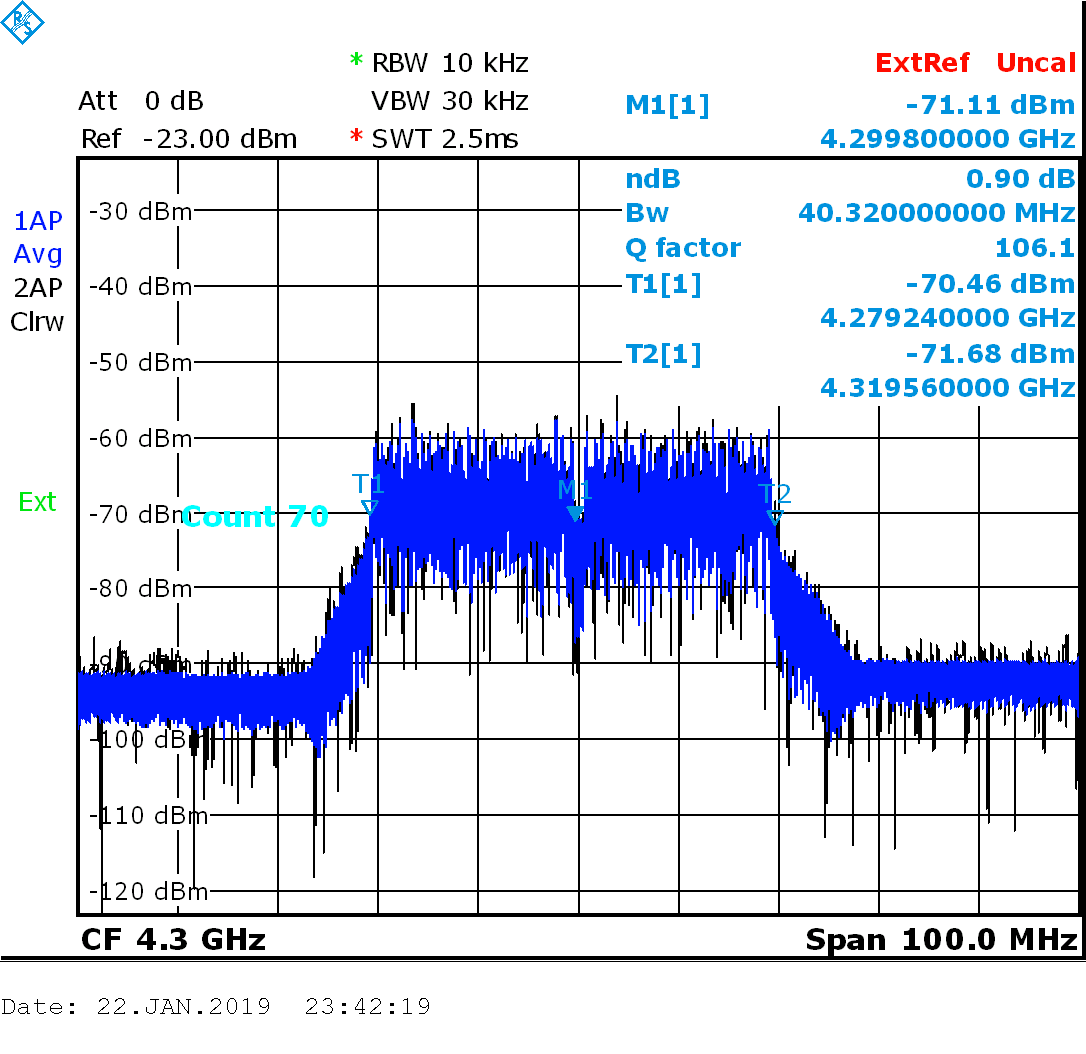
\includegraphics[scale=0.25]{ofdm_wvfrm.png}
\caption[]{MSK Waveform at 4.3 GHz Pictured on a Spectrum Analyzer}

\label{fig:OFDM}

\end{figure}
One way to view the OFDM waveform is as a series of MSK waveforms spread out orthogonally along a desired bandwidth. From this perspective, MSK can be seen as the minimum bandwidth version of a system based on OFDM, and the altimeter can thus be subjected to wider and wider bandwidth systems to show the response to a greater number of WAIC devices on an aircraft. This aspect, as well as the similarity of an OFDM signal to LTE systems made it a very attractive option for testing the impact of WAIC. 

Generating OFDM signals with the VSG was a more involved process than generating MSK, because the functionality for creating OFDM was not available natively in the VSG software. Because of this, OFDM had to be generated through the VSG's \textit{Arbitrary Waveform Generator}. The arbitrary waveform generator enables the VSG to generate any waveform from IQ data stored in a file on the VSG. The SCPI command for generating an arbitrary waveform would need to include the file path for this IQ data.  

This enabled an OFDM waveform to be specified by a Matlab script which exports raw IQ data, which is then converted to a form readable by the VSG through proprietary Rhode and Schwarz software. The conversion software allowed the user to adjust the clock rate, thus adjusting the bandwidth of the signal used. The bandwidth could then be measured with a spectrum analyzer to verify the process has yielded the expected waveform. The bandwidth of the OFDM waveform was defined as being 6 dB down from the peak power. 


\subsubsection{Dual Waveforms}\label{subsub:Dual}
The VSG allows full control of an RF generator along with two baseband generators. The RF generator gives the user control of RF carrier frequency as well as the output power level of the carrier in dBm. The baseband generators allow the modulation of two potentially unique waveforms onto the carrier wave, with a possible offset frequency from the center. Both dual MSK waveforms and dual OFDM waveforms of bandwidth less than 40 MHz were tested using a +/-20 MHz offset between them. 

Dual waveforms were considered an important option for testing due to a special characteristic of some altimeters at low altitudes. As the plane descends, the sweep rate of an altimeter increases to give more frequent readings at a more safety critical phase of flight. This is done by significantly reducing the $\Delta f$ covered by the altimeter FMCW. The effects of this offset were thus investigated to determine whether WAIC's impact could be minimized at critical altitudes by leaving the center of the band clear. 

\section{Python Test Software}\label{sec:Python}
Python code written by the author pieces together the various parts of this setup into a complete test bench. Different Python scripts handle different functions necessary to the test bench. These include:

\begin{itemize}
\item Creating a database to transfer data between different Python Scripts
\item Interface with the VSG to generate interference signals
\item Parse the CoPilot log
\item Mapping time stamped height measurements to time stamped interference signals
\item Plotting and analyzing the results
\end{itemize}

\begin{figure}[ht]
\centering
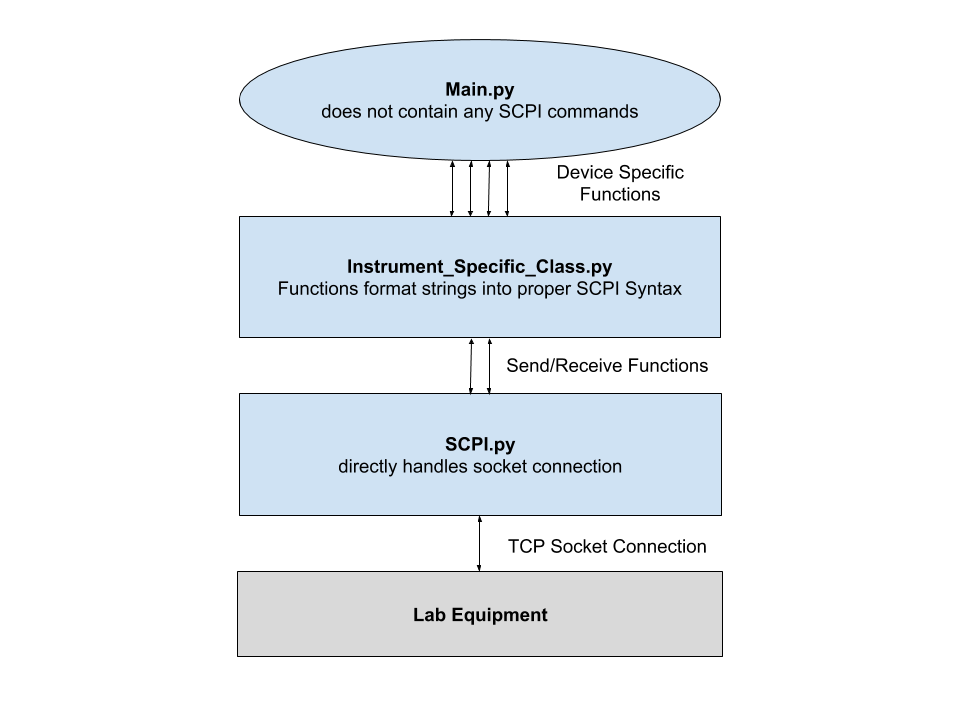
\includegraphics[scale=0.45]{SCPI_Class_Hierarchy.png}
\caption[]{SCPI Class Hierarchy}

\label{fig:SCPI}

\end{figure}
The software uses Standard Commands for Programmable Instruments or SCPI to control the vector signal generator. In this test bed, the SCPI instructions are processed through an object-oriented hierarchy shown in Figure~\ref{fig:SCPI}. The super-class, $SCPI$ interfaces directly with all lab equipment. The subclass, called \textit{RS\_Signal\_Generator} in this implementation, contains python functions associated with all instrument specific commands. The helper functions from $SCPI$ send and receive communication with the instrument. Finally, the main loop exists at the highest level, which times the calls of different instrument commands and creates a database to store them. 

\subsection{Test Main Loop}\label{sub:mainloop}
The highest level of this design is the test main loop. The test main loop creates the SQLite database which stores all important information for easy transfer between the different python scripts necessary for the test bed. This program also contains variables for various test parameters, which are stored in an SQLite database for easy reference and sometimes directly control the sequence of a test. Finally, this program loops through the sequence interference signals specified by the various test parameters, and sends the commands to the VSG to generate them. The commands sent to the VSG are time stamped as precisely as possible, and recorded in the \textit{Generated Signals} table in the database. 


Certain test parameters are stored for reference or calculation but do not directly affect the sequence of interference signals to be generated. These include the altimeter make and model, the nominal height of the test setup, the loss experienced by interference signals traveling to the altimeter RX, and the loop loss used in the setup. Other parameters directly control the sequence of the test, including interference on and off times, power levels to be used, modulation formats to be tested, and RF carrier frequencies to be used. 

\subsubsection{Nominal Height vs Correct Height}\label{subsub:nominal}
\textit{Nominal height} is the term used to refer to the height of the test setup. For example, the smallest spool of fiber optic cable is 500ft long, so the test setup using only this spool in the altitude simulator has a \textit{nominal height} of 500ft.  However, the measured height in a particular setup will typically differ from the nominal height by a small amount.  This small offset varies between the different altimeters under test. The difference between measured height and the nominal height of the setup can be attributed in part to the extra cabling going to and from the altitude simulator, but primarily is a result of different calibration settings for each altimeter. 

The calibration procedure is an important part of installing an altimeter onto an aircraft. When an aircraft is on the ground, the TX and RX antennas used by the altimeter are naturally several feet off the ground, in line with the airframe. To compensate for the varying heights of airframes, avionics manufacturers developed a calibration procedure so that each altimeter could be programmed upon installation to output an altitude of 0ft when the plane is on the ground. Because these tests are only concerned with \textit{height error}, rather than the most precise height measurement possible in the setup, this calibration is not corrected for in test procedures. Instead, a variable called \textit{correct\_height} is calculated in post processing as the median altitude with no interference. Any height error attributable to interference is measured as a distortion from this correct height.

\subsubsection{Sequence Control}\label{subsub:sequence}
% This section also needs a plot to show the timed stepping up of interference signals. 
The primary purpose of the test main loop is to subject an altimeter to various modulation formats, gradually stepping up the power of each until the altitude readings from an altimeter are distorted or broken. The main loop determines the type of modulation, power level, and timing, and as each signal is turned on or off by the VSG, stores the parameters for the signal in the \textit{Interference Signals} table for use in post processing, an example of which is shown in Table ~\ref{tab:Interference}. Each unique modulation format and power combination will have two entries in the \textit{Interference Signals} table, corresponding to the RF ON and RF OFF states of the VSG.  

A variety of parameters controls the progression of different interference signals. The \textit{interference\_duration} and \textit{signal\_off\_duration}, define the length of time the altimeter will be subjected to a particular interference signal, as well as the length of time the altimeter will have to recover from any error caused by the previous signal. Throughout the main loop, each signal's Start Time and End time is calculated using interference duration variables. 

 A range of RF powers is specified using \textit{power\_min}, \textit{power\_max}, and \textit{power\_step}. For a given modulation format, the main loop iterates through each power level in this range, subjecting the altimeter to this interference power. This allows the user to step through increasing power with as much granularity as is desired for the test

\begin{table}[]
\centering
\begin{tabular}{@{}cccccccc@{}}
\toprule
ID & Altimeter   & Start Time          & End Time            & Modulation &Carrier Freq& Power & RF State \\ \midrule
1  & Alt A & 19:23:06 & 19:23:07 & MSK & 4300  MHz & -10  dBm & OFF      \\
2  & Alt A & 19:23:07 & 19:23:08 & MSK & 4300   MHz & -10 dBm& ON       \\ \bottomrule
\end{tabular}
\caption{Example Interference Signals Table}
\label{tab:Interference}
\end{table}

The final variable which is important to the progression of a test is a list called \textit{modulation\_formats}, which contains strings corresponding to the different modulations the VSG will generate. MSK and OFDM signals of varying bandwidths will be listed here. The main loop iterates through each string in this list, passing the string to helper functions. 

The first helper function is a lookup which calls the proper function in the VSG class corresponding to a specific modulation format string. The second helper function gives the option for different modulation formats to be put on different carriers, or a list of different carrier functions. Iterating through different carriers for different modulation formats proved to be a critical functionality in later tests.

\subsubsection{Precision of Timing Commands}\label{subsub:timing}
During initial tests of the main loop, problems occurred which prevented the \textit{interference\_duration} and \textit{signal\_off\_duration} from precisely controlling the duration and recovery time of an interference signal. This section provides an overview of the different timing issues encountered over the course of these tests, as well as the approaches taken to mitigate each issue. 
 
The first and most serious issue encountered while running these tests were termed \textit{hanging delays}. These occurred when the main loop progressed more or less as expected, but the vector signal generator would ''hang'' in its previous state for a significant period of time after the command was sent. 



% Please add the following required packages to your document preamble:
% \usepackage{booktabs}
\begin{table}[]
\centering
\begin{tabular}{@{}ccccccccc@{}}
\toprule
ID & Timestamp   & RF State & Power  & PEP  & Carrier  & Offset 1 & Custom 1 & Arb 1 \\ \midrule
1  & 11:49:39.96 & 1        & -3 dBm & 4.48 & 4300 MHz & 0        & 0        & 1     \\
2  & 12:09:40.26 & 0        & -3 dBm & 4.48 & 4300 MHz & 0        & 0        & 1     \\ \bottomrule


\end{tabular}
\caption{Example VSG State Table}
\label{tab:VSG_State}
\end{table}
 
	 First, the program was modified and a new table was added to the database to store the Vector Signal Generator state after each set of commands. Since the purpose of this table was only to be used for debugging, entries were kept as simple as possible. For example, a $1$ in \textit{RF State} corresponds to RF ON, while conversely a $0$ in \textit{RF State} corresponds to the RF OFF setting. The \textit{Power} and \textit{Carrier} columns correspond with the same values in Table~\ref{tab:Interference}. \textit{Offset 1}, \textit{Custom 1}, and \textit{Arb 1} correspond to the state of the first Baseband generator, telling whether the \textit{Custom Waveform Generator} corresponding to a MSK Waveform (see Section~\ref{subsub:MSK}) or the \textit{Arbitrary Waveform Generator}(see Section~\ref{subsub:OFDM}) corresponding to an OFDM waveform are active respectively. 
	 
For the purposes of the timing problem, these attributes serve as a fingerprint, allowing an investigator to correlate each row in the VSG State Table to a row in the Interference Signals table. While information here may seem redundant, this value differs notably from the values in the interference signals table in that the VSG state table is only populated \textit{with values received from the Vector Signal Generator}. Because of this, this table allows for a simple method for looking through the data to find at which point the VSG might ''hang'' in its current state rather than switch to the next signal as specified in the interference signals table. 

Using this method, different theories for potential causes of the hanging delays were investigated. The first potential problem was dropped or delayed packets. During the initial setup, instruments were connected to one another over the TAMU network. While this functioned at a high level, upon packets had an unnecessarily long mean travel time, and significant outliers existed during times of heavy traffic. These issues were solved by moving the VSG and controller laptop onto their own local network. 

 While the local network solved the biggest chunk of hanging delays, it did not eliminate them entirely. These were attributed to a slowdown in the processor handling the sequence of Python commands.These remaining delays would only occur at times of extremely heavy CPU usage (caused by a memory leak in the old Ballard driver), and were eliminated almost completely by rebooting the controller laptop more frequently. Later on, an upgrade to the Ballard driver reduced these even further. 
 
 While the hanging delays were investigated, the VSG State table revealed another source of imprecision in timing commands. It was noticed that the VSG State would not change until nearly a second longer than the \textit{Interference Duration} or \textit{Signal off Duration} parameters specified. This drift occurred because the main loop used Pythons in built \textit{Sleep()} function to handle timing. The sleep function used the exact interference duration passed as a parameter. After the program 'woke up' the commands to set the next interference signal up would be called, thus introducing a small delay beyond the specified duration. 
 
 This problem was dealt with by replacing the \textit{Sleep()} function with a custom function called \textit{Wait\_Until()}. This new function takes the signal end time as a parameter (See Table ~\ref{tab:Interference}), subtracts the current time from the end time, and uses the new value as the parameter for Python's in-built sleep function. This allows the next end time to be calculated in advance by adding the \textit{Interference Duration} or \textit{Signal off Duration} to the previous signal's end time, and storing the previous signal's end time as the start time for the next signal. [This section definitely could use some sort of diagram...]

Using the \textit{wait until} method to time commands offered important new flexibility to the main loop. This method allows writing signals to a database, setting up the baseband generators, and pinging the VSG for the VSG State information all to occur while the VSG is in an RF OFF state. While the VSG settings can not be adjusted in RF ON while maintaining the integrity of the signal, writing to the database and pinging the VSG for state information can also be done during this state, and the \textit{wait until} function will still wake the program at the proper time to turn the VSG on or off. The implementation of the \textit{wait until} function eliminated the drift problem, and allowed for the \textit{Interference Duration} and \textit{Signal Off Duration} parameters to precisely control the signal on and off time. 

\begin{figure}[ht]
\centering
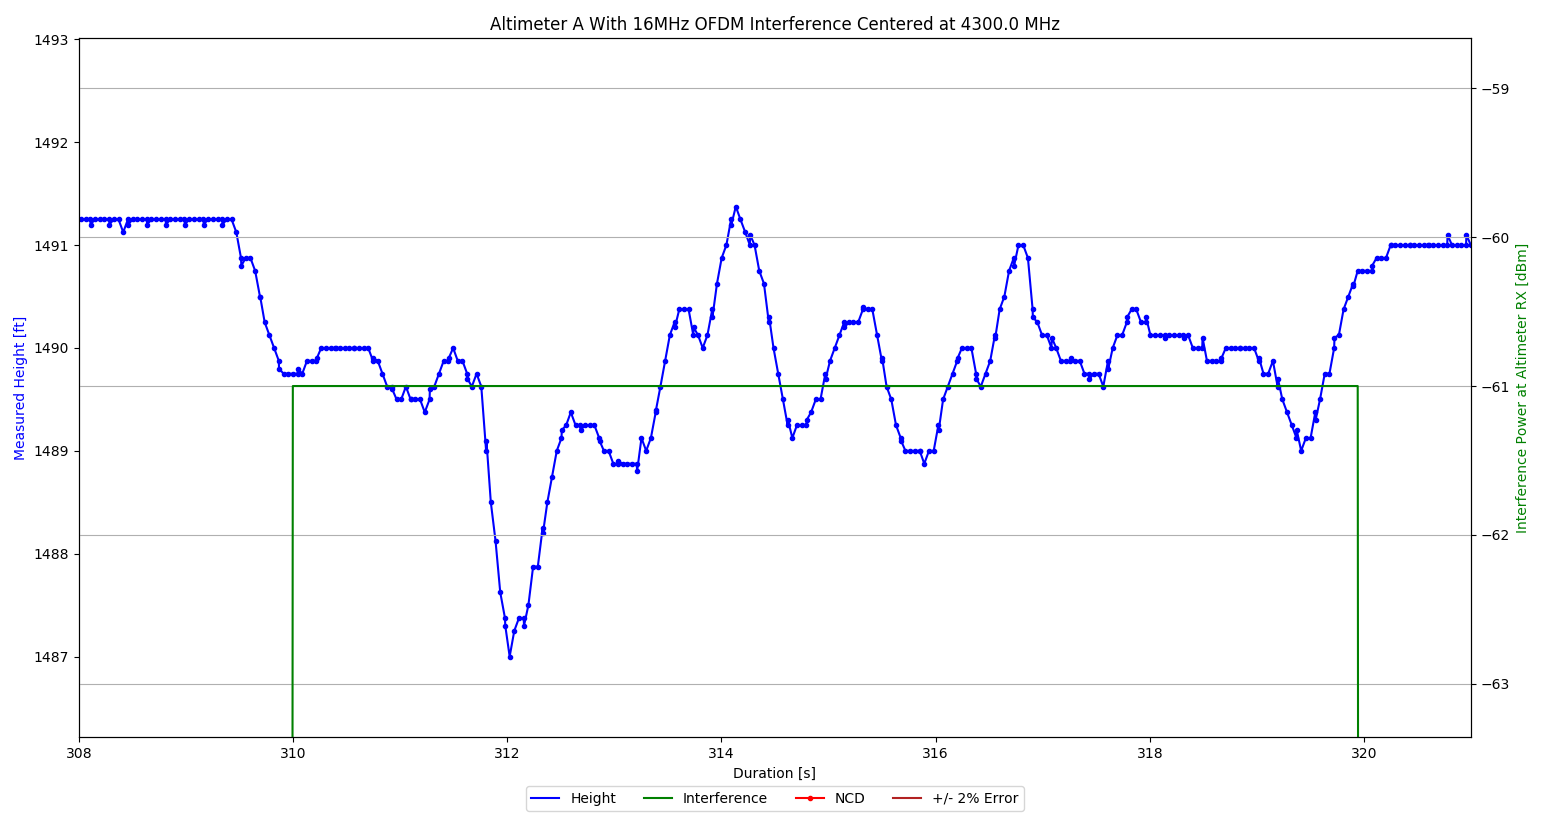
\includegraphics[scale=0.65]{sync_err.PNG}
\caption[]{Height Plot Showing Sync Error}

\label{fig:sync}

\end{figure}
The final problem encountered involved the synchronization of time stamps of data between the controller laptop and the Ballard ARINC device. The Ballard internal clock drifted from about half a second ahead of the controller laptop clock to about half a second behind. This led to data sets such which looked like Figure~\ref{fig:sync}, where distortion from the correct height would appear a split second before the interference signal was turned on. Additionally, due to averaging techniques used in the altimeter's signal processing, there would be several data points during which the altitude would recover from the distortion caused by any interference. 


While this issue could not be fixed completely, several different approaches were taken to mitigate it. Firstly, the Ballard used in initial testing was an older unit, which meant it was more prone to clock errors. To address this, the clock was driven by an external IRIG signal, rather than the on board IRIG. A program called NMEA time generated the IRIG signal through the controller laptop's audio jack, which was then fed into the Ballard input.  These changes would not completely synchronize the Ballard, but it would limit the drift of one clock away from another throughout a test. 


Later on, when a new Ballard was purchased for this project, the external IRIG signal was no longer needed, as the updated Ballard driver provided adequate synchronization over USB. Another technique used to prevent any loss of synchronization was to periodically power cycle the Ballard to ensure that the clock is reset. Finally, to minimize the impact of any data points not captured in the RF ON interval by post processing, long interference durations were used to ensure that the impact of any missed points on the true average was minimized. 

\subsection{VSG Class}
The VSG Class allows the main loop to create an object corresponding to each VSG connected to the network in the lab setup. This object then has access to functions which perform every operation needed by the main loop. The VSG Class inherits functionality from \textit{SCPI.py} common to every SCPI programmable instrument. 


\subsection{SCPI Class}
\subsection{Post - Processing}
After the test sequence is completed, a series of other Python scripts are used to post process the newly generated data. Time stamped altitudes must be exported from the Ballard CoPilot software into an Excel document, and a python script has to read the data from this log into the SQLite database. A second program uses the time stamps from both the logged altitude table and the generated signals table to create a full data set, where each altitude measurement is labeled with the type and magnitude of interference the altimeter was subjected to at that time. Finally, several Python scripts take this full dataset and use it to generate plots which aid in the interpreting of the results. 
\subsubsection{Parsing The Copilot Log}
\subsubsection{Mapping Interference Signals to Copilot Data}
\subsubsection{Plotting the Data}


\section{Setup for Testing Wider Bandwidth Interference}
This section covers how the Modified setup from Figure~\ref{fig:Modified} is again changed to allow for Wider Bandwidth OFDM signals, with the primary goal being to fill the entire 200 MHz altimeter band with simulated WAIC Interference. A secondary goal of this process is to test the effects of proposed Cellular networks in adjacent bands to the altimeter band while still maintaining simulated WAIC Interference. 

\section{Setup for WAIC plus Altimeter Interference}
This section covers another set of modifications to the setup from Figure~\ref{fig:Modified}, which are designed to simulate the interference from other altimeters. The test scenario of an aircraft approaching an airport (and thus other altimeters) was determined to be the most critical. A set of Voltage Controlled Oscillators (VCO's) were controlled by function generators with a waveform similar to that seen in Figure~\ref{fig:FMCW}.

%	\subsection{Calibrating the VCOs}

%\subsection{Handling Multiple Vector Signal Generators}
